\chapter{Background} \label{chap:relatedwork}

% --------------------- Volume rendering ---------------------
\section{Volume rendering} \label{sec:volumerendering}
Volume rendering is a technique for visualizing 3D data sets, such as those obtained from medical imaging scans. It works by computing a 2D projection of a 3D volume, using algorithms to assign colors and opacities to each point in the volume based on its physical characteristics, such as density or temperature. Many visual effects are volumetric in nature, e.g. fluids, clouds, flames, smoke, fog, and dust. These effects are challenging to simulate with geometric primitives like points, lines, triangles, or polygon meshes, and may be better simulated with volume rendering. A volume renderer may also be used to display not just the model's surfaces but all of its fine external and internal details, allowing the user to see inside the volume to get a better understanding of its internal structure. Because of this, volume rendering is a powerful tool for visualizing complex 3D data and can be used in a wide range of applications, including medical imaging, scientific visualization, and computer graphics\cite{max_optical_1995}.

%Volume rendering is a technique for visualizing 3D data sets, such as those obtained from medical imaging scans. It works by computing a 2D projection of a 3D volume, using algorithms to assign colors and opacities to each point in the volume based on its physical characteristics, such as density or temperature. A volume renderer may be used to display not just the model's surfaces but also all of its fine external and internal details, allowing the user to see inside the volume to get a better understanding of its internal structure. Many visual effects are volumetric in nature, and it is challenging to simulate fluids, clouds, flames, smoke, fog, and dust using geometric primitives. Such effects may be produced more effectively with volumetric models. \cite{ikits_chapter_2007}. Volume rendering is a powerful tool for visualizing complex 3D data and can be used in a wide range of applications, including medical imaging, scientific visualization, and computer graphics\cite{max_optical_1995}.

%"Direct volume rendering refers to techniques which produce a projected image directly from the volume data, without intermediate constructs such as contour surface polygons" \cite{max_optical_1995}. It makes it possible to project 2D images from a series of discretely sampled 3D data. A volume renderer may be used to display not just the model's surfaces but also all of its fine details. Many visual effects are volumetric in nature. It is challenging to simulate fluids, clouds, flames, smoke, fog, and dust using geometric primitives. Such effects may be produced more effectively with volumetric models. These models presuppose that a high number of particles in the volume emit, absorb, and scatter light \cite{ikits_chapter_2007}.

%After having acquired a 3D data set, rays are cast from the center of the viewing direction (camera origin), through the image plane and into the volume. As the ray enters the volume, an intensity profile is generated. The scalar value per the depth of the volume will be proportional with the density of the volume being traversed.
%Volume rendering enables photorealistic novel view synthesis \cite{xieNeuralFieldsVisual2022}.

There are multiple ways of rendering a volume. Well-known techniques include ray casting or raymarching, resampling or shear-warp, texture slicing, and splatting. The basic algorithm, visualized in \autoref{fig:volume-rendering}, can be broken into four steps:

\begin{itemize}
    \item \textbf{Ray casting:} Cast rays from the image plane into the volume. The volume is often enclosed within a bounding primitive like a cuboid.
    \item \textbf{Sampling:} As the ray enters the volume, sample equally spaced points from the volume. This equidistant sampling builds an intensity profile for the ray, density per volume depth. In the general case where the volume isn't aligned with the ray's direction, the sampling point will be positioned in between voxels, and the values must be interpolated from its adjacent voxels.
    \item \textbf{Shading:} Utilizing the generated intensity profile and a transfer function, we compute the $RGB\alpha$-color and an illumination-value gradient. The gradient vector points in the direction of the greatest increase, indicating where the most rapid increase in illumination is. The samples are colored with their $RGB\alpha$ value and shaded according to the gradient vector and the location of the scene's light source.
    \item \textbf{Compositing:} The final color of the pixel is retrieved by compositing all the shaded samples along the ray. 
\end{itemize}

\begin{figure}[h]
    \centering
    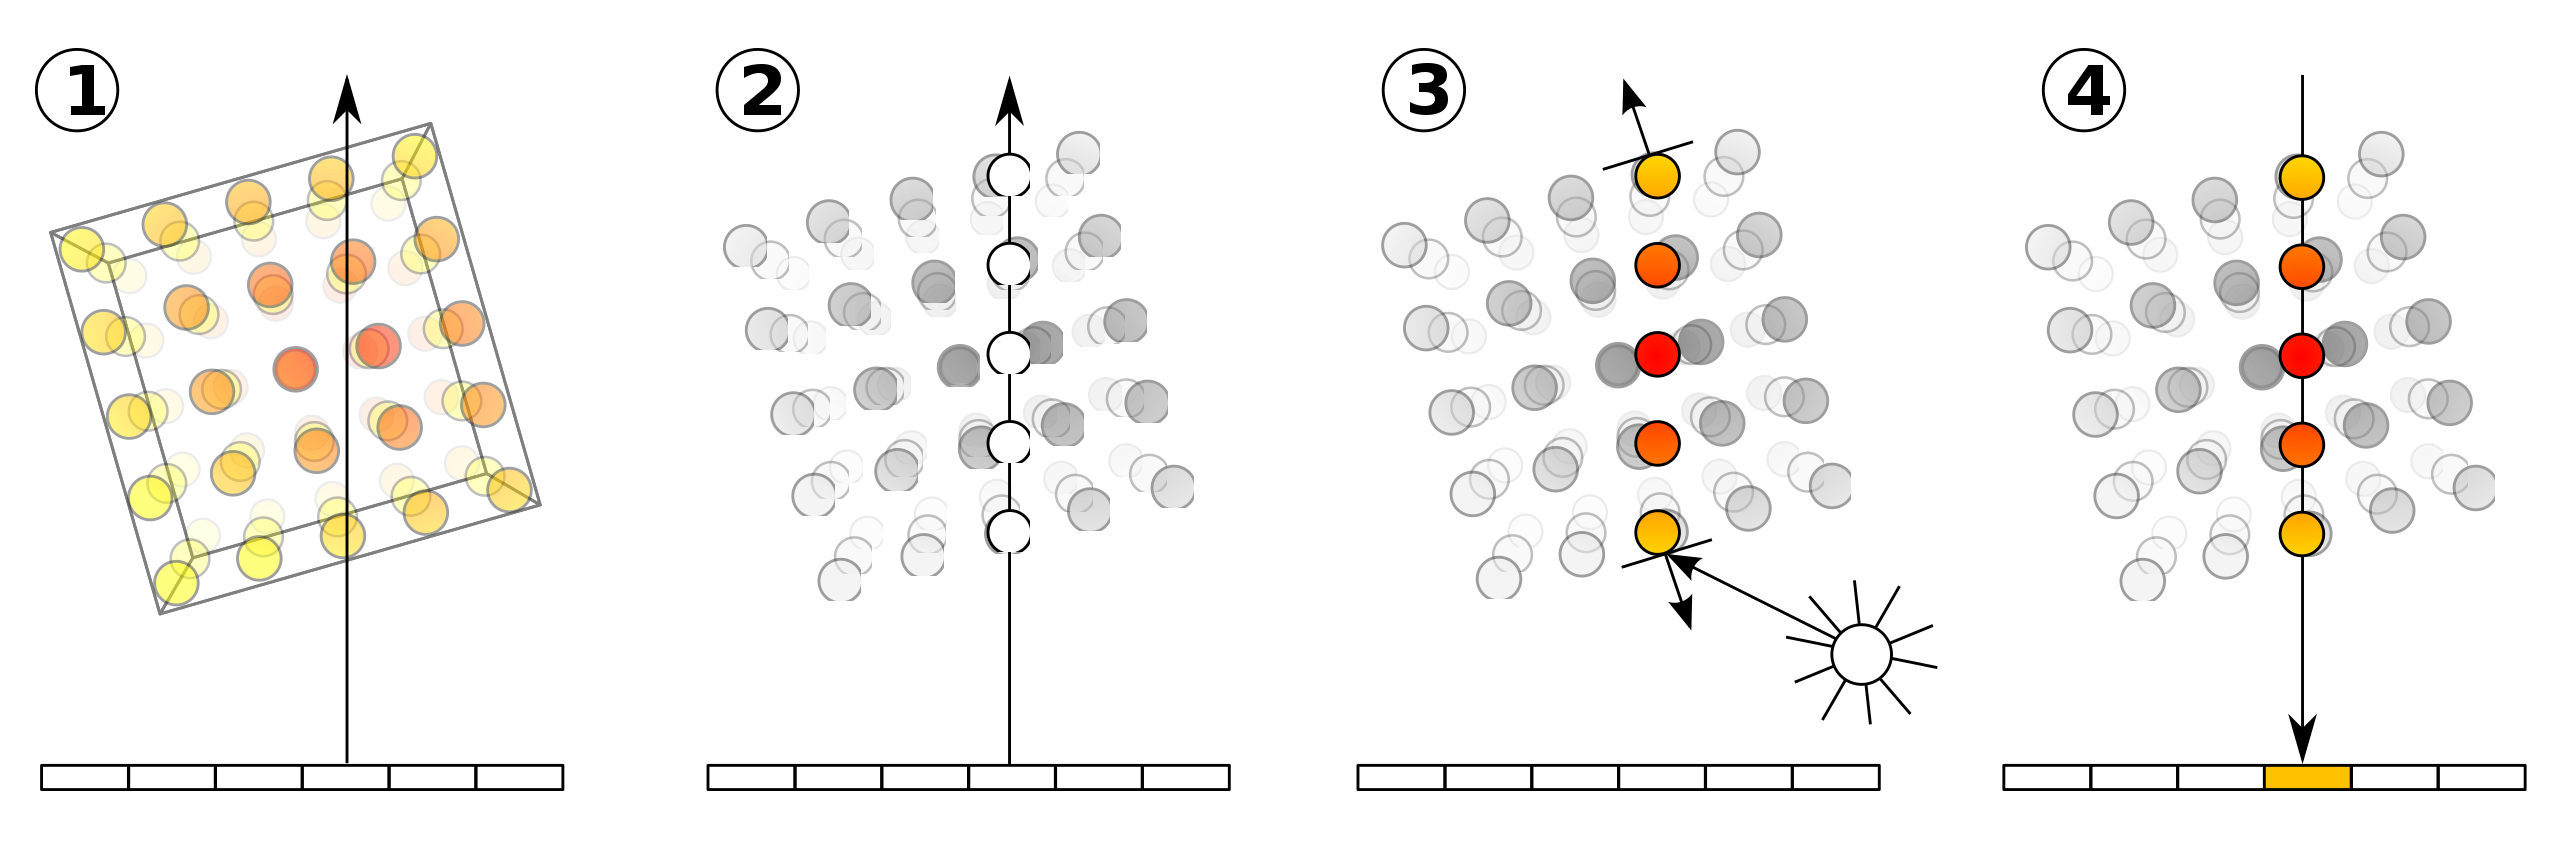
\includegraphics[width=1.0\textwidth]{figures/volume-rendering.png}
    \caption{The four basic steps of volume rendering \cite{wiki:Volume_ray_casting}. 1) A ray is cast from the image plane into the volume. 2) Points in the volume are sampled. 3) The points are shaded based on their $RGB\alpha$-value and the illumination-value gradients in relationship with the local light source. 4) The final pixel color is composited along the ray.}
    \label{fig:volume-rendering}
\end{figure}

\begin{comment}
\subsection{Alpha compositing}
Alpha compositing is the process of combining one image with a background to create the appearance of partial or full transparency \cite{wiki:Alpha_compositing}.

\subsection{Ray marching}
\end{comment}



% --------------------- Neural Fields ---------------------
\section{Neural Fields} % All text is taken from \cite{xie_neural_2022} - rewrite - have now paraphrased it
A field that has been entirely or partially parameterized by a neural network is known as a neural field. The field is a quantity that may be defined for any set of temporal or spatial coordinates. By design, neural fields are both continuous and adaptable. The parameterization of neural fields as MLPs with gradient-defined activation functions is common\cite{xie_neural_2022}.

A typical neural fields algorithm in visual computing would first, across space-time, sample coordinates and feed them into a neural network to produce field quantities. The field quantities are samples from the desired reconstruction domain of our problem. Then, we apply a forward map to relate the reconstruction to the sensor domain (e.g. RGB image), where supervision is available. Finally, we calculate the reconstruction error or loss that guides the neural network optimization process by comparing the reconstructed signal to the sensor measurement.



% --------------------- Neural Radiance Fields (NeRFs) ---------------------
\section{Neural Radiance Fields (NeRFs)}
Most of the volumetric data we interact with through computer games, movies, and other computer graphic applications, are represented by meshes. A mesh is a collection of vertices, edges, and faces that can be combined in order to define the shape of objects. Meshes are easy to manipulate and interact with. Another common representation of volume is voxels, where a 3D point in space is represented by a value, e.g. a color. Both of these modeling techniques are explicit representations. As we want to increase the resolution of a scene, we have to model increasingly smaller regions of space, i.e. increase the number of voxels/triangle-meshes in the volume. This doesn't scale well as the memory requirements increase as we increase the number of voxels/triangle-meshes. We have to find another way to represent the scene, instead of representing it as explicit blocks in space. NeRF provides an implicit representation of the scene by utilizing a multi-layered perceptron (MLP).

NeRF is a neural volumetric representation. The name, neural radiance fields, gives us a clue as to what it is. It is a field, a space full of particles, where each particle has a given radiance, a color emitted by the particle in a certain direction, and the field is represented with a neural network. NeRF parameterizes 3D scenes as 3D neural fields, mapping 3D coordinates to radiance and density. The 3D scene can subsequently be rendered via volume rendering \autoref{sec:volumerendering}.

\subsection{Differentiable rendering} % Change this - a lot directly from the paper
NeRFs are made possible due to differentiable rendering, a major breakthrough in 3D reconstruction. It allows reconstruction of 3D neural fields representing shape and/or appearance given only 2D images, instead of 3D supervision. Differentiable rendering has significant implications as 3D often is expensive to obtain, while 2D images are omni-present. Suddenly, non-experts can become 3D content creators, without the barrier of specialized hardware; an important social implication\cite{xieNeuralFieldsVisual2022}.

%A major breakthrough in 3D reconstruction was the adoption of differentiable rendering (Section 4), which allowed reconstruction of 3D neural fields representing shape and/or appearance given only 2D images, instead of 3D supervision. This has significant implications since 3D data is often expensive to obtain, while 2D images are omni-present. A particularly important social implication is that non-experts can become 3D content creators, without the barrier of specialized hardware. \cite{xieNeuralFieldsVisual2022}



% --------------------- NeRF ---------------------
\section{NeRF - Representing Scenes as Neural Radiance Fields for View Synthesis}
\begin{figure}
    \centering
    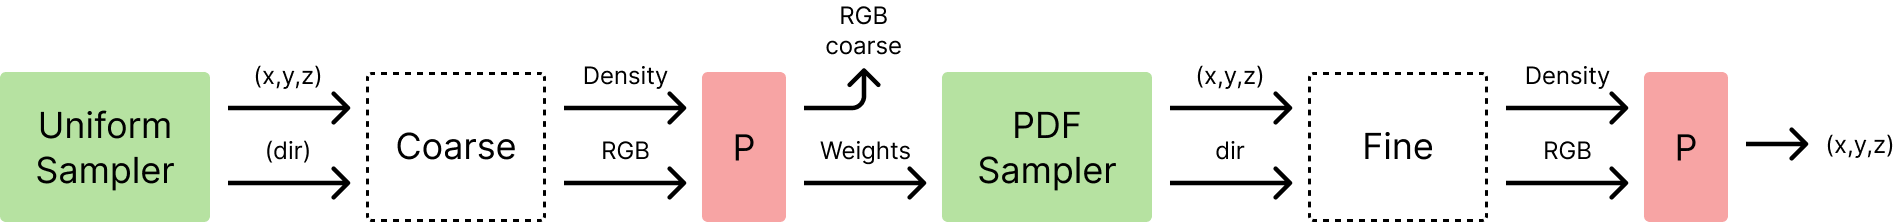
\includegraphics[width=1.0\textwidth]{figures/NeRF_Pipeline.png}
    \caption{Visualization of the NeRF pipeline}
    \label{fig:nerf-pipeline}
\end{figure}
The first paper to present Neural Radiance Fields (NeRFs) was \cite{mildenhall_nerf_2020}. NeRFs provides a method for reconstructing 3D scenes and synthesizing novel views. Given multiple 2D images and their corresponding camera poses, NeRF builds a dataset by sampling points in the volume. The points in the dataset are passed through an MLP in order to predict the given points' density and color. The predicted density and color values are then composited into a final color which is compared to the reference image pixel's color. The MLP is optimized to minimize the difference between the predicted and reference pixel color.

%NeRF does this by querying an underlying MLP overfit to a specific scene, which represents a continuous volumetric field.
%NeRF renders pixels by emitting rays into the scene. The rays are represented by the ray equation $\pmb{r}(t) = \pmb{o} + t\pmb{d}$ where $\pmb{o}$ is the ray's origin, usually the center of the camera, and $\pmb{d}$ is the ray's direction.

Given multiple 2D images and their corresponding camera poses, which can be approximated with Structure from motion techniques as discussed in \autoref{sec:sfm}, NeRF builds a dataset by sampling points in the volume. Points are sampled along a ray $\pmb{r}(t)$ with origin $\textbf{o}$, the camera's center of projection, and direction $\textbf{d}$. As discussed in \autoref{sec:hierarchicalsampling}, the original paper leverages hierarchical sampling to increase the sampling rate of important parts of the volumetric scene.

%Sample points along a ray $\pmb{r}(t)$, defined by the ray function \autoref{eq:ray-equation}.

\begin{equation}
    \pmb{r}(t) = \pmb{o} + t\pmb{d}
    \label{eq:ray-equation}
\end{equation}

%$\pmb{o}$ is the origin and $\pmb{d}$ is the ray's direction. 

A point $\pmb{x} = \pmb{r}(t_k)$ where $t_k \in t$ is a 3D-coordinate. These 3D coordinates, in conjunction with their viewing direction \textbf{d}, make up the dataset that the MLP is trained on. It's been shown that MLPs have a hard time learning high-frequency signals given low-dimensional input \cite{tancik_fourier_2020}. In order to remedy this, we normalize $\textbf{x}$ to lie in the interval of $[-1, 1]$ and increase the signals' dimensionality by applying positional encoding, \autoref{sec:positionalencoding}. The dimensionality of $\pmb{x}$ and its corresponding viewing direction $\pmb{d}$ is increased by applying $\gamma(\cdot)$ \autoref{eq:positionalencoding} to both.

\begin{equation}
    \gamma(p) = [\sin(\pi p), \cos(\pi p), ..., \sin(2^{L-1}\pi p), \cos(2^{L-1}\pi p)]^T
    \label{eq:positionalencoding}
\end{equation}

A predicted color can be retrieved by passing the encoded 3D coordinate and its corresponding encoded camera pose through the MLP $F_{\theta}$. The output of $F_\theta$ is a 4D vector containing a color $RGB$ and a density $\sigma$. In order to retain multiview consistency, NeRF first predicts the volume density $\sigma$ as a function of just the location $\textbf{x}$. Subsequently, the RGB color $\pmb{c}$ is predicted as a function of both the location and viewing direction.


Using the points' density $\sigma$ and color $\pmb{c}$ we can approximate the volume rendering, as discussed in \autoref{sec:volumerendering}, to synthesize a novel view of the scene. The expected color $C(\pmb{r})$ can be derived by \autoref{eq:volume-rendering}, which further can be approximated with numerical quadrature as shown in \autoref{eq:numerical-quadrature-loss}.

%Feed $\gamma(x)$ and its corresponding encoded camera pose given by $\gamma(\theta)$ and $\gamma(\phi)$ into the MLP $F_{\theta}$

\begin{equation}
    C(r) = \int_{t_n}^{t_f}T(t)\sigma(\pmb{r}(t))\pmb{c}(\pmb{r}(t), \pmb{d})dt \quad T(t) = \exp{\left(-\int_{t_n}^{t_f}\sigma(\pmb{r}(s))ds\right)}
    %C(r) = \int_{t_n}^{t_f}T(t)\sigma\pmb{c}dt \quad T(t) = \exp{(-\int_{t_n}^{t_f}\sigma ds)}
    \label{eq:volume-rendering}
\end{equation}
\begin{align} \label{eq:numerical-quadrature-loss}
    \hat{C}(\pmb{r}) = \sum_{i=1}T_i \alpha_i \pmb{c}_k, && \text{where}~T_i &= \exp{(-\sum_{j=1}^{i-1} \sigma_j \delta_j)},  \\ 
    && \alpha_i &= (1-e^{-\sigma_i}), \\ 
    && \delta_i &= t_{i+1} - t_i
\end{align}

The transmittance $T(t)$ can be viewed as the probability that the ray doesn't "hit anything", i.e. if the ray continues up until point $t$ or not. $\sigma(\pmb{r}(t))$ and $c(\pmb{r}(t), \pmb{d})$ is the density and color of point $\pmb{r}(t)$, respectively.

Since volume rendering is differentiable, we optimize the loss between the synthesized and ground truth observed image. This is done by calculating the total squared error between the ground truth pixel colors and the synthesized pixel color over all the rays $\pmb{r} \in \mathcal{R}$. Both the coarse and fine networks, as described in \autoref{sec:hierarchicalsampling}, are optimized over.

\begin{equation}
    L = \sum_{\pmb{r} \in \mathcal{R}} \left[\left\| \hat{C}_c(\pmb{r}) - C(\pmb{r}) \right\|^2_2 + \left\| \hat{C}_f(\pmb{r}) - C(\pmb{r}) \right\|^2_2\right]
    \label{eq:nerf-loss}
\end{equation}

An overview of the NeRF pipeline can be viewed in \autoref{fig:nerf-pipeline}

\subsubsection{Positional Encoding} \label{sec:positionalencoding}
Positional encoding is one of the many proposed encoding schemes, first introduced in the original NeRF paper. It is a method used to increase the dimensionality of an input vector, as it's shown that deep networks are biased toward learning lower-frequency functions. It is not to be confused with positional encoding in transformers. 

\subsubsection{Hierarchical sampling} \label{sec:hierarchicalsampling}
When training a NeRF, different sampling strategies can be utilized. The sampling strategy is an important choice as it is core to how the dataset for the MLP is constructed. In the original NeRF paper they used a sampling strategy called hierarchical sampling. The key notion is that they trained two MLPs, one \textit{coarse} and one \textit{fine}. The coarse MLP uses stratified sampling, as described in \autoref{sec:stratifiedsampling}, where points along the ray are sampled in uniform intervals within each bin. When being trained, the coarse MLP outputs a probability distribution function (PDF) of which samples contributed highly to the final predicted RGB value. This PDF is then passed to the fine MLP which sample points along the ray in accordance with the PDF. This strategy of having a coarse network predict the important areas to sample, i.e. the areas that contain a volume, helps the fine network predict a better result. \cite{mildenhall_nerf_2020}

% Point from Mip-NeRF 360. Doesn't fit very well here, but it's a good point!
%The only reason why the coarse network is supervised is to guide the sampling of the fine network. This is the motivation behind improvements in e.g. Mip-NeRF 360

\subsubsection{Stratified sampling} \label{sec:stratifiedsampling}
Stratified sampling is a sampling method. It has proven benefits in machine learning as it helps prevent overfitting. The sampling method consists of two steps:

\begin{itemize}
    \item \textbf{Partition the dataset into strata:} In the case of NeRF, a strata is the points contained within a bin $\pmb{x} \in [t_i, t_i+1]$ along the ray $\pmb{r}(t)$. The population/size of a strata can vary based on predefined functions. Importance sampling can be achieved by increasing the size of the strata in accordance with a PDF.
    \item \textbf{For each stratum, apply simple random sampling:} 
\end{itemize}

\begin{figure}[h]
    \centering
    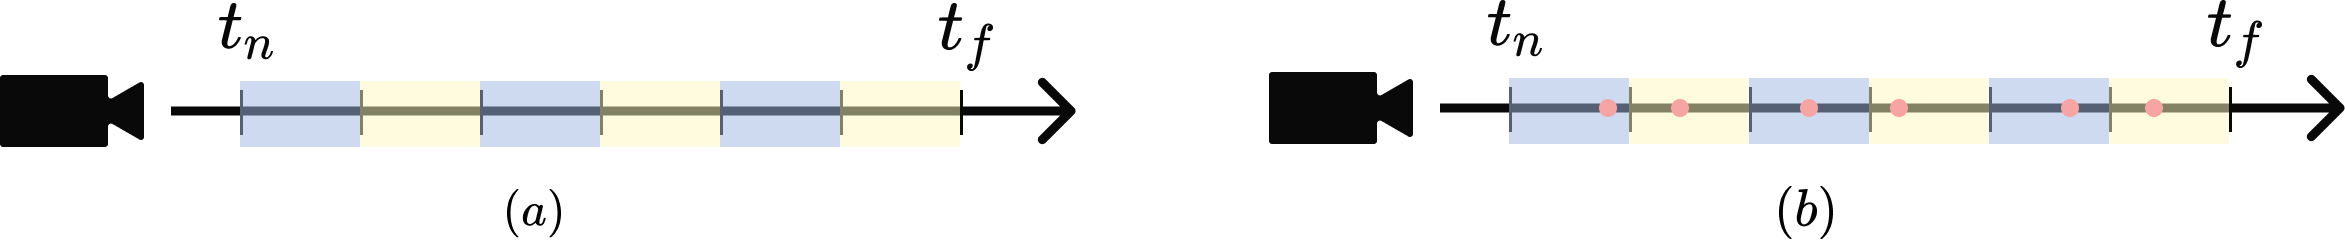
\includegraphics[width=1.0\textwidth]{figures/stratified-sampling.png}
    \caption{a) The ray is uniformly binned from the near bound $t_n$ to the far bound $t_f$, defining the strata. b) random points are sampled from the bins.}
    \label{fig:stratified-sampling}
\end{figure}





% --------------------- Other models that Nerfacto builds on ---------------------
% --------------------- mip-NeRF ---------------------
\section{Mip-Nerf} \label{sec:mipnerf}
\begin{figure}[h]
    \centering
    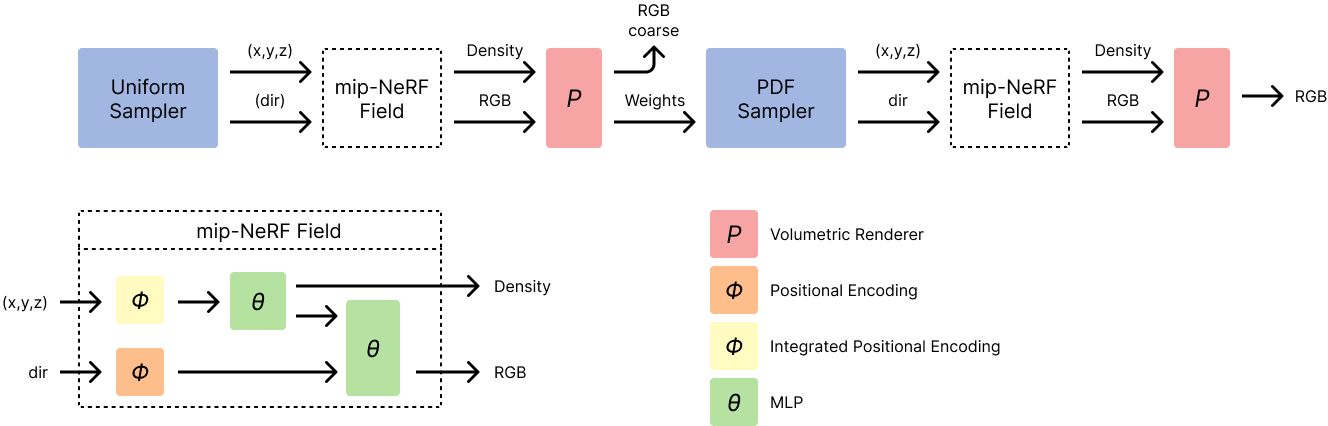
\includegraphics[width=1.0\textwidth]{figures/mip-nerf-pipeline-overview.png}
    \caption{}
    \label{fig:mip-nerf-pipeline-overview}
\end{figure}
NeRF shows good performance when all training and testing photos are taken at about the same distance from the scene, and it doesn't have to reason about scale or aliasing. When you add more cameras, pulled away from the scene, NeRF starts to break down, because it's a single-scale model now trying to solve a multi-scale problem. Renderings from the NeRF will show aliasing artifacts in distant views and excessive blur in close-up views.

A solution to this problem would be to adapt a solution that is used in offline ray tracing, supersampling. With supersampling, we would march multiple rays through the same pixel's footprint. This technique doesn't solve the issue of aliasing effects, but the rendered image would look better. However, doing so would be very computationally expensive and it would increase the already very long training times of NeRF, which already depends on querying an underlying MLP hundreds of times for a single ray.

Another sampling strategy apart from casting rays through each pixels' footprint would be to cast a cone, as seen in \autoref{fig:mip-nerf-frustums}. The cone's radius is determined by the size of the pixel's footprint on the image plane, so that the cone models the whole volume of space visible by the pixel. When the pixel's cone is rendered, all the content within that visible volume will be averaged out, instead of rendering out whatever intersects with the infinitely narrow ray that was cast by NeRF. The cone is divided into conical frustums. The frustums are approximated with a multivariate Gaussian since they're easier to manipulate and have a closed-form solution.

\begin{figure}[ht]
    \centering
    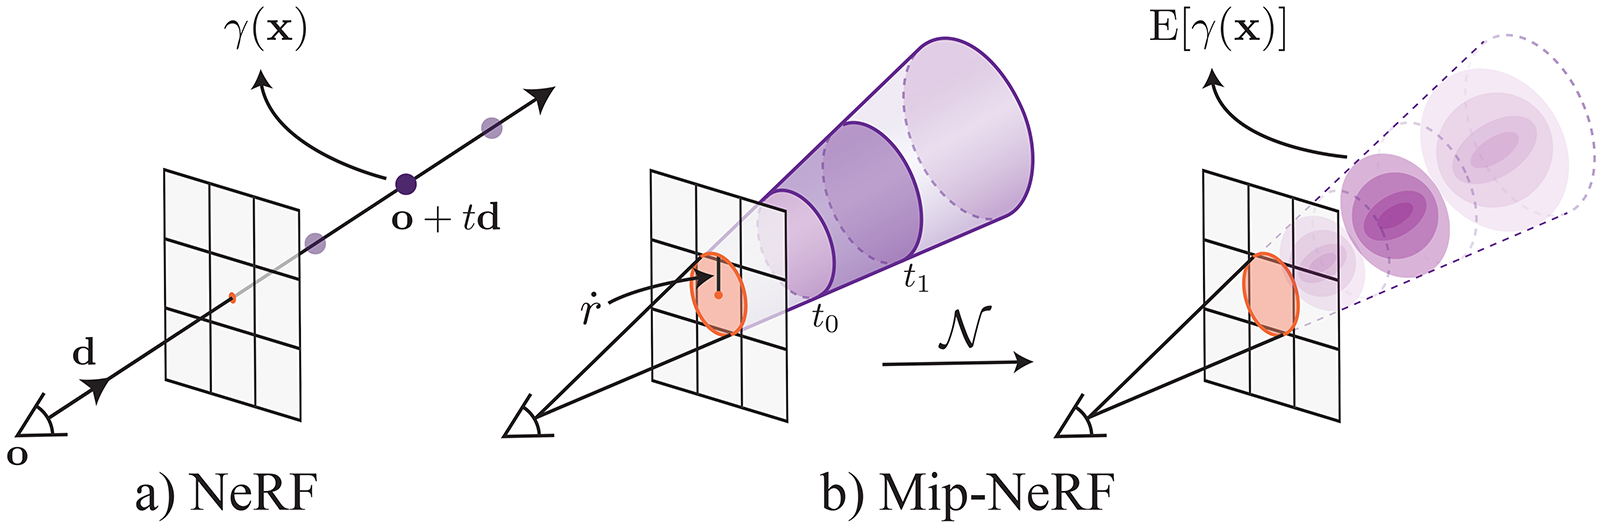
\includegraphics[width=1.0\textwidth]{figures/mip-nerf-frustums.png}
    \caption{Figure 1 from Mip-NeRF \cite{barron_mip-nerf_2021}. Cones are cast through the pixels' footprint and into the volume.}
    \label{fig:mip-nerf-frustums}
\end{figure}

Instead of positionally encoding a single point along the ray, we compute the expected positional encoding with respect to the Gaussian that we've constructed. With this encoding, mip-NeRF is able to reason about the scale of its input by looking at the scale of the encodings. This lets the model understand the difference between small and large volumes. This encoding scheme is called integrated positional encoding (IPE), and has a simple closed-form that can be computed quickly.

Inspiration to this method is taken from mipmapping which traditionally has been used to prevent aliasing in computer graphics pipelines. A mipmap is a pre-filtered set of discretely downsampled signals, very often images, which helps speed up rendering as the responsibility of anti-aliasing is shifted to a precomputation phase. Mip-NeRF extends NeRF to simultaneously represent the pre-filtered radiance field for a continuous space of scales, thereof "mip-NeRF".




% --------------------- mip-NeRF 360 ---------------------
\section{Mip-NeRF 360} \label{sec:mipnerf360}
\begin{figure}[h]
    \centering
    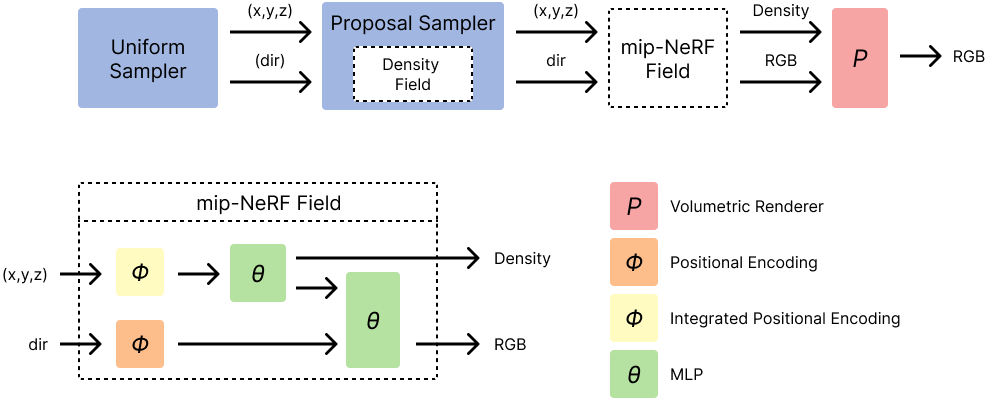
\includegraphics[width=1.0\textwidth]{figures/mip-nerf-360-pipeline-overview.png}
    \caption{}
    \label{fig:mip-nerf-360-pipeline-overview}
\end{figure}
Mip-NeRF provides a lot of helpful techniques in order to proceed with the evolution of NeRFs, but it focuses on forward-facing scenes instead of unbounded scenes; scenes with a main object of interest in front of an elaborate background. This is where Mip-NeRF 360 picks up, it addresses challenges with extending mip-NeRF to unbounded scenes. There are primarily three techniques proposed by Mip-NeRF 360 which we'll cover in this section.

\textbf{Representation}:
%Problem: Unbounded scenes are large, but mip-NeF needs a bounded domain
%Solution: Apply a Kalman-like warp to mip-NeRF Gaussians to warp the mip-NeRF into non-Euclidean space.
The first challenge with extending mip-NeRF to unbounded scenes is that unbounded scenes are large, but mip-NeRF requires a bounded domain. Mip-NeRF handles scenes unbounded in one direction by warping the space into projective space, normalized device coordinates (NDC), but the challenge arises when the scene is unbounded in all directions. A solution is to apply a Kalman-like warp to mip-NeRF Gaussians in order to warp the mip-NeRF into non-Euclidean space. All the Gaussians outside a sphere of radius one will smoothly be warped into a non-euclidean space within a sphere of radius two. This non-Euclidean space is used to represent the input to the MLP. 


\textbf{Efficiency:}
%Problem: Large scenes require more network capacity, but using a large MLP is too expensive (given that you have to query it hundred of times for a single ray)
%Solution: "Distill" scene geometry from a large NeRF MLP into a small MLP while training. Train a small proposal MLP to bound the geometry predicted by a large NeRF MLP which makes training ~3 times faster
Extending a bounded scene to an unbounded scene will lead to larger scenes. These scenes require more network capacity, but using a large MLP is too expensive given that you have to query it hundreds of times for a single ray. A solution is to distill scene geometry from a large NeRF MLP into a small \textit{proposal MLP} while training. The proposal MLP will only output a set of weights, no colors. By feeding a set of location points through the proposal MLP, the outputted weights can then be used as a PDF to resample the ray, the same way the coarse network in hierarchical sampling guides the fine network's sampling. The resampled points are then used to render a color, which as normal is supervised with photometric loss. Instead of supervising the proposal MLP to accurately reconstruct the image, which is done for both the coarse and fine MLPs in mip-NeRF, we supervise its output weights to be consistent with the output weights from the NeRF MLP. We do this with a loss function that encourages the outputted weight histograms, which have different bin endpoints, to be consistent with one another. This is possible due to some strong assertions on the relation between the two distributions, summarizing the same underlying, true distribution. This new approach to training accelerates training by 300\%.

%i.e. calculate a loss that correlates the output weights from the NeRF MLP and the proposal MLP. Due to this we can have a very small proposal MLP which we query very frequently, and a larger NeRF MLP which is queried relatively few times.
%To make this work we need a loss function that encourages histograms with different bin endpoints to be consistent with one another. To achieve this we make some strong assertions on the relation between the two distributions, summarizing the same underlying, true distribution. The loss function will penalize any excess mass that violates the upper bound imposed on the proposal MLP.


\textbf{Ambiguity:}
%Problem: 3D reconstruction becomes more ambigious as you increase the scene size. Results in more artifacts
%Solution: Utilize a novel regularizer designed specifically for mip-NeRF ray intervals. The regularizer encourages each ray's histogram to be as close to a delta function as possible. 
Reconstructing 3D content from 2D photos is inherently ambiguous since the content of unbounded scenes can be everywhere and will only be seen by a tiny number of rays. This problem increase as you increase the scene size. The original NeRF-paper partially addressed this behavior by introducing random Gaussian noise to the output $\sigma$ values, before passing them through the ReLU. It stimulated densities to drift toward either zero or infinity, which slightly enhanced visual performance. This regularization isn't sufficient for the more challenging task mip-NeRF 360 seeks to tackle. Instead, they utilize a novel regularizer, designed specifically for mip-NeRF ray intervals, that encourages each ray's histogram to be as close to a delta function as possible. This regularizer reduces the occurences of "floaters", semi-transparent material floating in space.



\section{Block NeRF}
Block NeRF is a paper that demonstrates a method for large-scale reconstruction of scenes using NeRFs. It does this by splitting large areas into multiple blocks of a certain radius, where each block has a connected NeRF, dubbed a block-NeRF. The different block-NeRFs are trained on images within their radius of responsibility. At inference time, only the block-NeRFs with a radius that spans the requested location are kept. These are all trained on image data from the requested location and can render an output. Some of the remaining block-NeRFs might still be without a direct line of sight to the requested location, which results in low "visibility". These block-NeRFs are also filtered out, resulting in a pool of block-NeRFs with good visibility. The color outputs of the remaining block-NeRFs are merged to render the final image output.

Block NeRF leverages multiple techniques in order to enable the reconstruction of large scenes.

\subsection{Appearance embeddings} \label{sec:appearance-embeddings}
Per image appearance conditioning is a technique proposed for NeRFs in \cite{martin-brualla_nerf_2021} and later used in multiple implementations. The appearance embeddings help reduce artifacts from the scene, especially "ghosting" artifacts which present themselves as fog in the final render. The appearance embedding is a vector in a low-dimensional space, unique for every input image, that is optimized jointly with the NeRF in order to allow the NeRF to process and represent 3D scenes with variable lighting, exposures, weather, and post-processing effects. In order to accommodate for these variations, we condition the final part of the MLP by passing the viewing direction concatenated with the appearance embedding. 
%The appearance embedding is concatenated with the viewing direction and passed through an MLP 

\subsection{Learned pose refinement} \label{sec:camera-pose-refinement}
Camera pose refinement is a technique proposed for NeRFs on forward-facing scenes in \cite{wang_nerf--_2022}. It has later been built upon to support imperfect camera poses for full 3D scene representations in \cite{lin_barf_2021}. Block-NeRF leverages pose refinement on large unbounded scenes. It is a technique proposed to reduce the impact of imperfect camera poses. In NeRF, this can be done by treating the camera poses and intrinsics as learnable parameters and jointly optimizing them with the 3D scene representation, i.e. optimizing both the photometric loss and the corresponding camera poses. Pose refinement is a very effective measure to reduce cloudy artifacts and increase the sharpness and overall quality of the resulting 3D representation.

\subsection{Visibility prediction}
Visibility prediction is done in order to predict if a given point is within the line of sight of a specific block-NeRF. The prediction is done by a secondary MLP $F_v$ that is trained to learn an approximation of the visibility of a sampled point. Given a location and a viewing direction, $F_v$ outputs an approximation of that location's transmittance ($T$ in \autoref{eq:volume-rendering}). The transmittance of a location will be close to 1 if it's visible, i.e. located in free space or on the surface of the first intersected object. Objects inside or behind the first intersected object will have a transmittance close to 0. If the point is seen from multiple viewing directions, the resulting transmittance will be the average of these observations. $F_v$ is supervised by the block-NeRF's main MLP $F_\sigma$.



% --------------------- Instant-ngp ---------------------
\section{Instant-ngp}
I should probably cover Insant-ngp too.



% --------------------- Structure from motion ---------------------
\section{Structure from motion} \label{sec:sfm}
Structure from motion is a technique for estimating 3D structures from sequences of 2D input images. In NeRF it is used a preprocessing tool for retrieving camera poses of the input images. In most NeRF methods, accurate camera poses are a strict requirement, although some papers have experimented with removing the need for pose supervision \cite{lin_barf_2021}.

\subsection{COLMAP} \label{sec:colmap}
COLMAP is a general-purpose Structure-from-Motion (SfM) \cite{schoenberger2016sfm} and Multi-View Stereo (MVS) \cite{schoenberger2016mvs} pipeline. The general overview of the pipeline contains the following steps:
\begin{itemize}
    \item Feature detection and extraction
    \item Feature matching and geometric verification
    \item Structure and motion reconstruction
\end{itemize}

During the first step, SIFT-features \cite{Lowe2004} are extracted. Sparse feature points in the image are found and their appearences are described using numerical descriptors.

% TODO: Elaborate on the different match-options; Exhaustive Matching, Sequential Matching, Vocabulary Tree Matching. Runtimes, found in the paper, can be added to appendix.

During the second step, features are matched. Correspondences between the feature points are matched across different images, leveraging feature matching and geometric verification. There are different options for matching algorithms. Exhaustive matching would match every image against every other image, leading to the best reconstruction results. The time complexity is not an issue if the number of images are relatively low (several hundreds). Another option is sequential matching which is useful if the captured images are in sequential order, e.g. if they're sampled from a video.

During the third step, structure and motion is reconstructed. First COLMAP will generate a sparse reconstruction of the scene, extracting the camera poses. The sparse output serves as input to the Multi-View Stereo to recover a dense representation of the scene. The dense representation estimates the dense surfaces. As COLMAP is used as a preprocessing step for retrieving the camera poses of input images, the pipeline is usually ceased after the sparse reconstruction.

\begin{table}[h] 
\centering
\begin{tabular}{lcc}
\hline
Matching algorithm & \multicolumn{1}{l}{Time complexity} & \multicolumn{1}{l}{Space complexity} \\ \hline
Exhaustive         & $\mathcal{O}(n^2)$       & $\mathcal{O}(n^2)$  \\
Sequential         & $\mathcal{O}(n k)$ & $\mathcal{O}(n k)$        \\
Vocabulary Tree    & $\mathcal{O}(n^2)$       & $\mathcal{O}(n k)$  \\ \hline
\end{tabular}
\caption{An overview of the time and memory complexities of a selection of COLMAP matching algorithms. For sequential matching $k$ is the number of adjacent images each image $n$ is matched against. For Vocabulary tree-based matching, $k$ is the number of top-retrieved images that each image $n$ is matched against.}
\label{tab:colmap-feature-complexity}
\end{table}

\begin{comment}
Exhaustive matching:
time complexity: O(n^2), where n is the number of images
memory complexity: O(n) for storing all images, O(n^2) for storing the results of the matching process

Sequential matching:
time complexity: O(n * k), where n is the number of images and k is the number of adjacent images each image is matched against
memory complexity: O(n * k)

Vocabulary tree-based matching:
time complexity: O(n^2), assuming that the size of the vocabulary tree is constant and not a function of the number n of images
memory complexity: O(n * k), where k is the number of top-retrieved images that each image is matched against
There is definitively literature on the topic of the time and memory complexity of vocabulary tree-based matching and image retrieval
\end{comment}




% --------------------- Evaluating NeRFs ---------------------
\section{Evaluating NeRFs} \label{sec:evaluating-nerfs}
Evaluating the quality of NeRFs is inherently hard since it's a visual modality. After a NeRF is trained it will eventually be used to render an image. Image similarity metrics are consequently the most important metric to evaluate the quality of a NeRF. The assessment of image similarity has been a long-standing challenge in computer graphics, but the following metrics are commonly used throughout most papers comparing NeRFs.

\subsection{PSNR - Peak Signal-to-Noise Ratio}
PSNR is a common measure for quantifying reconstruction quality for images and videos. It builds upon MSE which measures the absolute difference between each pixel in two images $I_1$ and $I_2$.

\begin{align} 
    \text{PSNR} &= 20 \cdot \log_{10}\left(\dfrac{MAX_I}{\sqrt{\text{MSE}}}\right) \label{eq:psnr}, \ \text{where} \\ 
    %\\ &= 20 \cdot log_{10} (MAX_I) - 10 \cdot log_{10}(MSE)
    \text{MSE} &= \dfrac{1}{m n} \sum_{i = 0}^{m-1} \sum_{j = 0}^{n-1} \left[I_1(i,j) - I_2(i, j) \right]^2, \ \text{and} \label{eq:mse}
\end{align}

$MAX_I$ represents the dynamic range of an image, i.e. the highest pixel value that the picture may contain. This is 255 when pixels are represented with 8 bits per sample. In more general terms, $MAX_I$ is $2^B-1$ when samples are recorded with $B$ bits per sample. Due to the high dynamic range of many signals, PSNR is typically expressed as a logarithmic number using the decibel (dB) scale.

\subsection{SSIM - Structural Similarity}
Although MSE and PSNR are good measures of the reconstruction error, they don't examine an image the same way humans do. We don't compare pixel-value to pixel-value in order to conclude if two images are similar, we look at it in a more holistic way. SSIM tries to capture this by instead comparing luminance $l$, contrast $c$ and structure $s$ between two windows $x$ and $y$ of common size $N \times N$.

\begin{align} \label{eq:ssim}
    \text{SSIM}(x, y) &= l(x,y)^\alpha \cdot c(x,y)^\beta \cdot s(x,y)^\gamma \qquad \text{with } \alpha, \beta, \gamma = 1 \\
    &= \dfrac{(2\mu_x \mu_y + c_1)(2\sigma_{xy} + c_2)}{(\mu_x^2 + \mu_y^2 + c_1)(\sigma_x^2 + \sigma_y^2 + c_2)}
\end{align}

\begin{comment}
\begin{itemize}
    \item $\mu$ represents the pixel sample mean for both $x$ and $y$,
    \item $\sigma^2$ represents the variance for both $x$ and $y$,
    \item $\sigma_{xy}$ represents the covariance of x and y,
    \item $c_1 = (k_1L)^2$, $c_2 = (k_2L)^2$ are variables to stabilize the division with weak denominator,
    \item $L$ represents the dynamic range of the pixel-values,
    \item $k_1 = 0.01$, $k_2 = 0.03$ by default   
\end{itemize}
\end{comment}

SSIM is bounded by $-1 \leq \text{SSIM} \leq 1$ where $1$ implies perfect correlation, $0$ implies no similarity, and $-1$ implies perfect anti-correlation.

\subsection{LPIPS - Learned Perceptual Image Patch Similarity \cite{zhang_unreasonable_2018}}
LPIPS is a perceptual similarity metric based on deep network activations. Where MSE, PSNR and SSIM uses relatively shallow functions in order to determine similarity across images, LPIPS leverage deep neural networks to obtain a metric that perceives similarity the same way humans do. Image patches with a low LPIPS score are perceptually similar.

\begin{figure}[h]
    \label{fig:lpips}
    \centering
    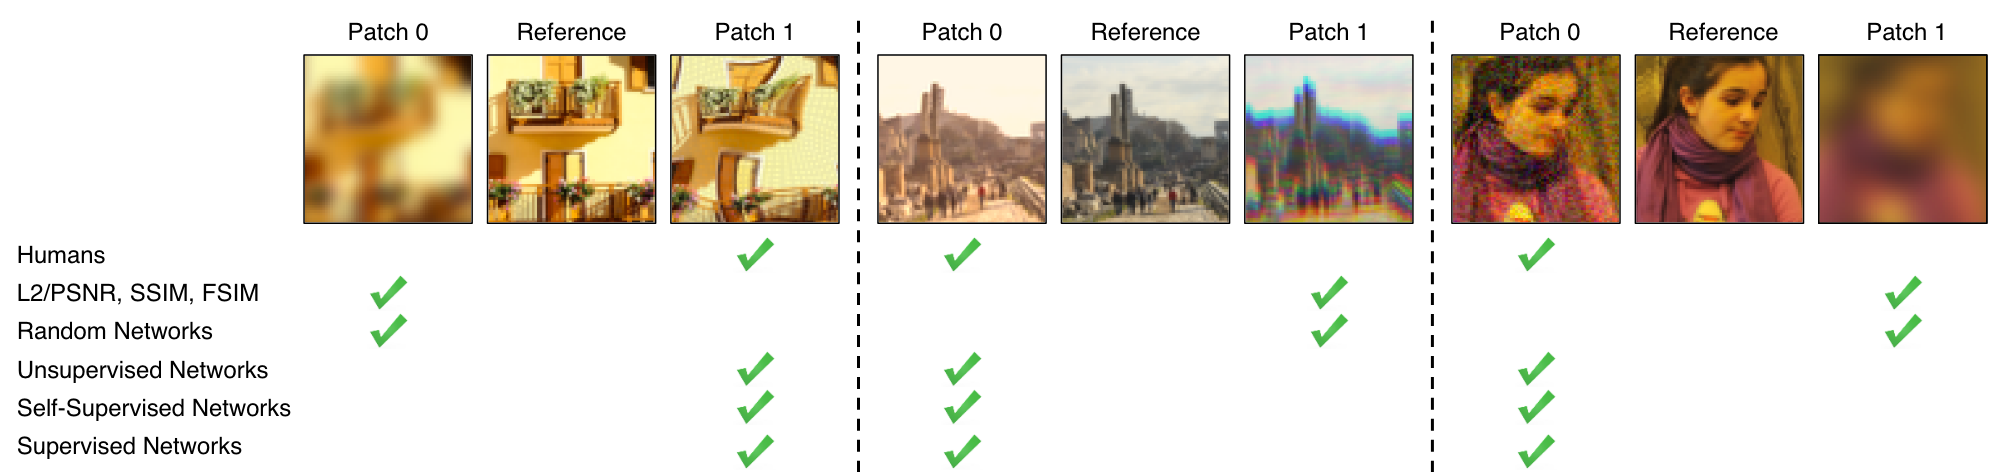
\includegraphics[width=1.0\textwidth]{figures/LPIPS.png}
    \caption{LPIPS is trained to perceive image similarity the same way humans do. The dataset used to train the similarity metric contains two types of perceptual judgements, Two Alternative Forced Choice (\pmb{2AFC}) and Just Noticeable Differences (\pmb{JND}). With 2AFC people were asked to select which of the distorted images was "closer" to the reference. With JND people were presented with 2 image patches, one reference and one distorted, and asked if they were the same.}
    \label{fig:my_label}
\end{figure}

%The metric determines how similar two image patches' activations are, for a given network. It's been demonstrated that this metric closely matches human perception. Image patches with a low LPIPS score are perceptually similar.

